\documentclass[12pt,a4paper]{report}

\usepackage[a4paper,left=2.55cm,right=2.55cm,top=2.6cm,bottom=2.8cm]{geometry}
\usepackage{amsmath,amssymb}
\usepackage{graphicx}
\usepackage{array,multirow}
\usepackage{enumitem}
\usepackage{caption}
\usepackage{float}
\usepackage{xcolor}
\usepackage{tikz}
\usetikzlibrary{arrows.meta,positioning,decorations.pathreplacing,calc}
\usepackage[export]{adjustbox}
% categorical colours, same fixed order as the plots
\definecolor{cBlue}{HTML}{2A78D6}
\definecolor{cOrange}{HTML}{EB6834}
\definecolor{cAqua}{HTML}{1BAF7A}
\definecolor{cYellow}{HTML}{EDA100}
\definecolor{cPink}{HTML}{E87BA4}
\definecolor{cInk}{HTML}{1F1F1E}
\newcommand{\diagram}[1]{\begin{adjustbox}{max width=\textwidth,center}\input{diagrams/#1}\end{adjustbox}}
\usepackage[hidelinks]{hyperref}

\linespread{1.2}
\captionsetup{font=small,labelsep=colon}
\captionsetup[table]{position=above,skip=6pt}
\renewcommand{\arraystretch}{1.1}
\graphicspath{{figures/}}

\newcommand{\reporttitle}{Catastrophic Forgetting in Continual Ear Recognition}
\newcommand{\authorname}{Harsh Chattar}
\newcommand{\rollno}{22CS30028}
\newcommand{\supervisor}{Prof. Debasis Samanta}
\newcommand{\semester}{Autumn Semester, 2026-27}
\newcommand{\reportdate}{November 6, 2026}

\begin{document}

% ------------------------------------------------------------------ title page
\begin{titlepage}
\centering
\vspace*{0.2cm}

\includegraphics[width=4.6cm]{iitkgp_logo.png}\\[0.8cm]
{\large\bfseries Department of Computer Science and Engineering\\
Indian Institute of Technology Kharagpur\\[0.9cm]}
{\huge\bfseries \reporttitle\par}
\vspace{0.8cm}
{\normalsize A Master's Thesis Project Report Submitted in Partial Fulfillment of the Requirements for the Dual Degree (B.Tech and M.Tech)\\[0.8cm]}
{\normalsize Submitted by\\[0.2cm]}
{\Large\bfseries \authorname\\}
{\small (\rollno)\\[1.3cm]}
{\normalsize Under the supervision of\\[0.3cm]}
{\Large\bfseries \supervisor\\[1.0cm]}
{\large \semester\\ \reportdate\\}
\end{titlepage}

% ------------------------------------------------------------------ declaration
\begin{center}
\vspace*{0.6cm}
{\Large\bfseries Declaration}
\end{center}
\vspace{1.6cm}
\noindent I certify that
\begin{enumerate}[label=(\alph*),itemsep=1.1em]
\item The work contained in this report has been done by me under the guidance of my supervisor.
\item The work has not been submitted to any other Institute for any degree or diploma.
\item I have conformed to the norms and guidelines given in the Ethical Code of Conduct of the Institute.
\item Whenever I have used materials (data, theoretical analysis, figures, and text) from other sources, I have given due credit to them by citing them in the text of the thesis and giving their details in the references. Further, I have taken permission from the copyright owners of the sources, whenever necessary.
\end{enumerate}
\vfill
\noindent
\begin{minipage}[t]{0.5\textwidth}
Date: \reportdate\\
Place: Kharagpur
\end{minipage}\hfill
\begin{minipage}[t]{0.45\textwidth}
\raggedleft
\textbf{\authorname}\\
(\rollno)
\end{minipage}
\vspace*{1.5cm}
\thispagestyle{empty}
\newpage

% ------------------------------------------------------------------ certificate
\begin{center}
\vspace*{0.5cm}
{\large\bfseries DEPARTMENT OF COMPUTER SCIENCE AND ENGINEERING\\
INDIAN INSTITUTE OF TECHNOLOGY KHARAGPUR\\
KHARAGPUR - 721302, INDIA\\[1.2cm]}

\includegraphics[width=4.6cm]{iitkgp_logo.png}\\[1.6cm]
{\large\bfseries CERTIFICATE}
\end{center}
\vspace{0.8cm}
\noindent This is to certify that the project report entitled ``\textbf{\reporttitle}'' submitted by \textbf{\authorname} (Roll No. \rollno) to Indian Institute of Technology Kharagpur towards partial fulfillment of requirements for the award of degree of Dual Degree (B.Tech and M.Tech) in Computer Science and Engineering is a record of bona fide work carried out by him under my supervision and guidance during \semester.
\vfill
\noindent
\begin{minipage}[t]{0.45\textwidth}
Date: \reportdate\\[0.6cm]
Place: Kharagpur
\end{minipage}\hfill
\begin{minipage}[t]{0.5\textwidth}
\raggedleft
\rule{\linewidth}{0.4pt}\\
\textbf{\supervisor}\\
Department of Computer Science and Engineering\\
Indian Institute of Technology Kharagpur\\
Kharagpur - 721302, India
\end{minipage}
\vspace*{0.8cm}
\thispagestyle{empty}
\newpage

% ------------------------------------------------------------------ abstract
\begin{center}
\vspace*{0.6cm}
{\Large\bfseries Abstract}
\end{center}
\vspace{0.6cm}
\noindent A deployed ear recognition system must enroll new people over time without being retrained from scratch. When a network is trained on new people one group after another, it tends to lose what it learned about earlier groups: this is catastrophic forgetting. This report does two things. First, it measures forgetting in a frozen, pre-registered benchmark: five model families (ResNet-50, ConvNeXt-T, MobileNetV3, DeiT-S and Swin-T) on four public ear datasets (AMI, AWE, IITD-I and EarVN1.0), each split into five tasks of new identities, with a jointly trained model as the upper bound. Under a strict rule that must hold on every seed, forgetting is shown in 9 of the 20 model--dataset cells: in all five families on EarVN, in three on AWE and in one on AMI; IITD shows none on rank-1. Learning without Forgetting and a small replay buffer cut EarVN forgetting by 0.17--0.29. Second, it tests whether the Continuum Memory System (CMS) of Nested Learning, placed in the pointwise layers of every backbone, reduces this forgetting. Against a decision rule committed before the runs, CMS reduced forgetting in none of the 9 cells (largest drop 0.036), and adding it to replay helped in none of 20. Diagnostics on EarVN ConvNeXt-T show that 93\% of the forgotten accuracy lies in exactly the layers CMS replaces, but that the slow memory copies moved only 0.4--1\% from their pretrained weights, against 10\% for the fast copy, because the adaptive optimizer normalises each slow update. Two exploratory variants, task-aligned update periods and explicit consolidation at task boundaries, reduced forgetting in 2 and 0 of the 9 cells. Catastrophic forgetting in ear recognition is real and model-independent on large datasets, and CMS as applied here does not fix it; the diagnostics point to how slow levels are updated as the part to change.

\vspace{1.4cm}
\noindent \textbf{Keywords:} \textit{Ear Recognition,\linebreak[1] Continual Learning, Catastrophic Forgetting, Nested Learning, Continuum Memory System, Biometrics.}
\thispagestyle{empty}
\newpage

% ------------------------------------------------------------------ acknowledgment
\setcounter{page}{4}
\chapter*{Acknowledgment}
I would like to express my sincere gratitude to my supervisor, Professor Debasis Samanta, for his invaluable guidance, support, and encouragement throughout this project. His review of the first phase of this work set the direction of the study reported here.

I would also like to extend my special thanks to my mentor, Santhoshkumar Peddi, for his continuous guidance and insightful suggestions, which greatly benefited my work.

\vfill
\begin{flushright}
\textbf{\authorname}\\
(\rollno)
\end{flushright}

\tableofcontents

% ================================================================== CHAPTER 1
\chapter{Introduction}

\section{Context}
The outer ear is a useful biometric. Its shape is distinctive, it stays stable through adult life, and it can be captured without contact and at a distance, often from the same camera that sees the face. Deep networks now dominate ear recognition, usually as a pretrained backbone fine-tuned to produce an embedding in which images of the same person lie close together \cite{emersic2017survey}.

A recognition system in use does not see all its people at once. New users are enrolled in batches: a new site, a new semester of students, a new group of employees. The obvious way to bring such a group into the model is to fine-tune on it. Neural networks trained this way tend to lose what they learned about earlier data, a failure known as \emph{catastrophic forgetting} \cite{mccloskey1989}. For a biometric system this means that people enrolled earlier are recognised less well after every update. The alternative, retraining on everybody each time, needs every past image to be kept, which is costly and often not allowed for biometric data.

\section{Research Gap}
Continual learning has a large literature \cite{delange2021survey}, but it is mostly about image classification on CIFAR or ImageNet subsets, where each new task brings new classes and the model is scored by a classifier head. Ear recognition differs in three ways. The model is used as an embedding: people are enrolled with gallery images and identified by similarity, so forgetting shows up as drift of the features, not as lost classifier weights. Ear datasets are small, from 100 to a few hundred people, and very different from each other in image quality. And it is not known whether forgetting depends on the model family, since most ear work uses one backbone.

Recently, \emph{Nested Learning} (NL) \cite{behrouz2025nested} proposed to view a network as a set of nested optimisation problems that update at different frequencies, and introduced a \emph{Continuum Memory System} (CMS): copies of an MLP block that are updated at different rates, so knowledge overwritten in a fast copy can survive in a slow one. NL reports reduced forgetting in class-incremental text classification with a pretrained language model. It has not been tested on vision backbones, on embedding models, or on biometrics.

\section{Scope and Objectives}
\subsection{Scope}
This report covers the second phase of the project. The first phase (B.Tech Project, Part I) studied few-shot ear recognition with meta-learning. Following the supervisor's review, the study was restarted on a narrower question: whether models forget when they learn new people one group after another, and whether Nested Learning reduces that forgetting. The study is limited to four public ear datasets, five ImageNet-pretrained backbones, and identity-incremental learning with five tasks per dataset. The fifth planned dataset, UERC 2023 \cite{emersic2023uerc}, was not finished in time and is left out.

\subsection{Objectives}
The study answers three research questions:
\begin{itemize}
\item \textbf{RQ1.} Do standard ear models from different families forget catastrophically when they learn new people one group after another?
\item \textbf{RQ2.} Does Nested Learning, in the form of a multi-frequency CMS, reduce that forgetting on exactly the same models, datasets and splits?
\item \textbf{RQ3.} Can Nested Learning be turned into a practical continual-enrollment method for ears?
\end{itemize}

\section{Approach}
Every dataset is its own experiment, and every comparison is made on the same frozen splits, task lists, input size, training budget and metrics. Each decision rule was written down and committed to the project's version history before the runs it judges, and each verdict was recomputed from the raw accuracy matrices by a separate script. The work is organised in stages: R0 freezes the benchmark; R1 tunes a recipe per model and dataset and trains the joint upper bound; R2 measures forgetting (RQ1); R3 tests CMS (RQ2); diagnostics explain the R3 result; and R4 and R4b are exploratory follow-ups towards RQ3 (Figure~\ref{fig:pipeline}).

\begin{figure}[H]
\centering
\diagram{pipeline}
\caption{Stages of the study, with the outcome of each. Blue stages were pre-registered; the orange stage is exploratory.}
\label{fig:pipeline}
\end{figure}

\section{Key Contributions}
\begin{itemize}
\item \textbf{A frozen continual ear recognition benchmark} across four datasets and five model families, with hash-pinned splits and task lists, open-set evaluation of seen people, and a pre-registered rule for when forgetting counts as shown.
\item \textbf{Evidence that forgetting is real and model-independent on large data:} all five families forget heavily on EarVN (rank-1 forgetting 0.33--0.48), while near-ceiling datasets hide it on rank-1.
\item \textbf{The first test of NL's CMS on vision backbones for biometrics,} with a pre-registered decision rule, giving a clear negative result.
\item \textbf{Diagnostics that locate the failure:} forgetting sits in the layers CMS replaces, but the slow copies barely learn, because an adaptive optimiser normalises their accumulated updates.
\item \textbf{Two exploratory CMS variants,} reported with the same test, which narrow down what would have to change.
\end{itemize}


% ================================================================== CHAPTER 2
\chapter{Background and Related Work}\label{ch:background}

\section{Ear Recognition}
Early ear recognition used hand-crafted descriptors on controlled images. Datasets collected ``in the wild'', such as AWE \cite{emersic2017survey}, showed that such descriptors fail under changes in pose, lighting and occlusion, and deep networks fine-tuned from ImageNet now perform best \cite{emersic2017survey,emersic2023uerc}. Most systems train an embedding and identify a probe by its nearest gallery identity. An angular-margin loss such as ArcFace \cite{deng2019arcface} is a common choice for training such embeddings, and it is used here. Ear recognition is usually evaluated with one network at a time, so it is not known how much the choice of backbone family matters for continual learning.

\section{Continual Learning and Catastrophic Forgetting}
In continual learning a model is trained on a sequence of tasks and should keep its performance on earlier tasks \cite{delange2021survey}. Here each task is a group of new people, which is the class-incremental setting \cite{vandeven2019three} applied to identities. Three families of methods are used as references in this study:
\begin{itemize}
\item \textbf{Regularisation.} Elastic Weight Consolidation (EWC) \cite{kirkpatrick2017ewc} penalises changes to weights that were important for earlier tasks, measured by the Fisher information.
\item \textbf{Distillation.} Learning without Forgetting (LwF) \cite{li2017lwf} keeps the new model's outputs on the current data close to those of the model before the task, without storing old images.
\item \textbf{Replay.} A small buffer of stored examples from earlier tasks is mixed into training \cite{rebuffi2017icarl,chaudhry2019tiny}. Replay is simple and very strong, but it stores biometric images, which may not be allowed.
\end{itemize}
Forgetting is measured from an accuracy matrix, as the drop from the best accuracy a task ever had to its final accuracy \cite{chaudhry2018riemannian}; backward transfer \cite{lopezpaz2017gem} is reported as well (Section~\ref{sec:metrics}).

\section{Nested Learning and the Continuum Memory System}
Nested Learning \cite{behrouz2025nested} describes a model as a set of nested associative memories, each solving its own optimisation problem with its own update frequency. Ordinary backpropagation layers, optimiser states and attention are all seen as memories that compress their own stream of data. A component updated rarely acts as a long-term memory; one updated every step acts as a short-term memory. NL builds on the earlier Titans memory module \cite{behrouz2025titans}.

\subsection{The Continuum Memory System}
CMS turns one MLP block into $k$ blocks with update frequencies $f_1 > f_2 > \dots > f_k$. Block $\ell$ is updated once every $C^{(\ell)}$ steps, with the sum of the gradients it accumulated over that period (NL, Eq.~71):
\begin{equation}
\theta^{(\ell)}_{i+1} =
\begin{cases}
\theta^{(\ell)}_{i} - \sum_{t=i-C^{(\ell)}}^{i} \eta^{(\ell)}_t \, \nabla \mathcal{L}\big(\theta^{(\ell)}_t; x_t\big) & \text{if } i \equiv 0 \pmod{C^{(\ell)}},\\[2pt]
\theta^{(\ell)}_{i} & \text{otherwise.}
\end{cases}
\label{eq:cms}
\end{equation}
The blocks can be chained, nested, or used independently and combined; in the independent variant (NL, Eq.~74) the output is an aggregate of all blocks,
\begin{equation}
y_t = \mathrm{Agg}\big(\mathrm{MLP}^{(f_1)}(x_t), \dots, \mathrm{MLP}^{(f_k)}(x_t)\big).
\end{equation}
The intended effect is that knowledge overwritten in a fast block survives in a slower one. NL also shows that the blocks can be initialised from a pretrained model's MLPs (NL, Sec.~7.3), which makes CMS usable on top of a pretrained backbone. In NL's experiments, CMS applied to the MLPs of a pretrained language model reduced forgetting in class-incremental text classification compared with EWC and other baselines. Its only vision result is an optimiser, not a memory in the network.

\section{Position of this Work}
No earlier work tests CMS on vision backbones, on embedding models, or for biometrics. This report applies the independent variant of CMS, initialised from pretrained weights, to the pointwise layers of five backbone families, and judges it with a rule fixed in advance against the same naive, EWC, LwF and replay baselines.

% ================================================================== CHAPTER 3
\chapter{Benchmark and Experimental Protocol}\label{ch:benchmark}

This chapter describes the frozen benchmark (stage R0). Everything in it was fixed and committed before any training run that is reported, and every later stage uses it unchanged.

\section{Datasets}
Four public datasets are used (Table~\ref{tab:datasets}). Each is a separate experiment: models never move from one dataset to another, so no cross-dataset identity overlap check is needed. Duplicate images within a dataset are removed when its file list is built. A fifth dataset, KinEar, was inspected and dropped, because its photos are uncropped phone pictures and some person folders are byte-identical copies of others. UERC 2023 \cite{emersic2023uerc} was prepared on the departmental GPU cluster, but its runs did not finish in time.

\begin{table}[H]
\centering
\small
\caption{Ear datasets used in the study.}
\label{tab:datasets}
\begin{tabular}{|l|c|c|l|}
\hline
\textbf{Dataset} & \textbf{People} & \textbf{Images} & \textbf{Character} \\
\hline
AMI \cite{gonzalez2012ami} & 100 & 700 & 7 per person, close-up, uniform size \\
AWE \cite{emersic2017survey} & 100 & 1,000 & 10 per person, in the wild, variable size \\
IITD-I \cite{kumar2012iitd} & 221 & 793 & 3--6 per person, grayscale \\
EarVN1.0 \cite{hoang2019earvn} & 164 & 28,412 & many per person, small images \\
\hline
\end{tabular}
\end{table}

\section{Identity-Incremental Tasks}
For each dataset and seed, 70\% of the people are training identities and the rest are kept for validation and test as never-seen people. The training identities are split into five tasks of equal size, so the model learns five groups of new people one after another (Table~\ref{tab:tasks}).

From each training person, some images are held out and never trained on. They measure how well the model still recognises people it has learned. On AMI and AWE, two held-out gallery images and one held-out probe are kept per person. On EarVN, 20\% of each person's images are held out. IITD has too few images per person, so only one probe is held out and the person's own training images serve as the gallery. This makes IITD's scores a little optimistic, but forgetting is still measured correctly, as a drop of the same score over later tasks. Figure~\ref{fig:protocol} summarises the protocol.

\begin{figure}[H]
\centering
\diagram{protocol}
\caption{The identity-incremental protocol. Training people are split into five tasks; each person keeps held-out images that are never trained on. After each task the model re-enrols every task's people and is tested on them, which fills one row of the accuracy matrix $A$.}
\label{fig:protocol}
\end{figure}

\begin{table}[H]
\centering
\small
\caption{Tasks and held-out images per dataset (seed 0).}
\label{tab:tasks}
\begin{tabular}{|l|c|c|c|c|}
\hline
\textbf{Dataset} & \textbf{Tasks $\times$ people} & \textbf{Train images} & \textbf{Gallery images} & \textbf{Held-out probes} \\
\hline
AMI & 5 $\times$ 14 & 280 & 140 (held out) & 70 \\
AWE & 5 $\times$ 14 & 490 & 140 (held out) & 70 \\
IITD-I & 5 $\times$ 31 & 400 & 400 (training images) & 155 \\
EarVN1.0 & 5 $\times$ 23 & 15,858 & 230 (held out) & 3,732 \\
\hline
\end{tabular}
\end{table}

Every split and task file is pinned by its MD5 hash, and the training script refuses to run if a file differs. Seed 0 is used only for tuning, on validation people. Seeds 1--3 are reported on every dataset; AMI, AWE and IITD also report seeds 4 and 5, because their per-task tests are tiny: with 14 probes per task on AMI and AWE, one probe moves a task's rank-1 by 0.07.

\section{Model Families}
Five ImageNet-1k-pretrained backbones from \texttt{timm} \cite{wightman2019timm} cover the main design families (Table~\ref{tab:models}). Only ImageNet-1k weights are used, so no model gets extra pretraining data. Stochastic depth is turned off for all of them.

\begin{table}[H]
\centering
\small
\caption{Model families and pretrained weights.}
\label{tab:models}
\begin{tabular}{|l|l|c|c|}
\hline
\textbf{Family} & \textbf{Model (timm weights)} & \textbf{Parameters} & \textbf{Feature size} \\
\hline
Classic CNN & ResNet-50 \cite{he2016resnet} (\texttt{tv2\_in1k}) & 23.5M & 2048 \\
Modern CNN & ConvNeXt-T \cite{liu2022convnext} (\texttt{fb\_in1k}) & 27.8M & 768 \\
Lightweight CNN & MobileNetV3-L \cite{howard2019mobilenetv3} (\texttt{ra\_in1k}) & 4.2M & 1280 \\
Plain transformer & DeiT-S \cite{touvron2021deit} (\texttt{fb\_in1k}) & 21.6M & 384 \\
Hierarchical transformer & Swin-T \cite{liu2021swin} (\texttt{ms\_in1k}) & 27.5M & 768 \\
\hline
\end{tabular}
\end{table}

\section{Training Setup}
All arms share one setup. Images are resized to 128$\times$96, which keeps the ear's aspect ratio and suits EarVN's small images; all five backbones accept this size, and \texttt{timm} resamples DeiT's position embeddings and Swin's attention-bias tables. The backbone feeds a neck that projects to a 512-dimensional embedding, trained with an ArcFace head ($s = 30$, $m = 0.3$) \cite{deng2019arcface}. Training uses AdamW \cite{loshchilov2019adamw} with weight decay 0.05, a head learning rate of $10^{-3}$, batch size 64, dropout 0.3, the same augmentation for all, and full fp32 precision. Precision is fixed because an earlier phase of the project found that mixed precision alone changes how much a model forgets.

The training budget is fixed as a rule rather than a number: it is counted in optimiser steps per task, tuned per model and dataset in R1, and then used unchanged by every sequential arm of that cell. The joint model trains for five times that number of steps on all people together. Steps are used rather than epochs because an AMI task has only 56 training images, a single step at batch size 64.

\section{Evaluation and Metrics}\label{sec:metrics}
After each task $t$, every task $j$ is evaluated: the held-out gallery images of task $j$'s people are enrolled with the \emph{current} model as cosine-similarity prototypes, and task $j$'s held-out probes are identified against them, together with a fixed set of probes from never-trained people. This gives an accuracy matrix $A[t][j]$, the score on task $j$ after training on task $t$. With $T = 5$ tasks, the summaries are:
\begin{align}
\text{Final} &= \frac{1}{T}\sum_{j=1}^{T} A[T][j], \\
\text{Forgetting} &= \frac{1}{T-1}\sum_{j=1}^{T-1} \Big(\max_{j \le t < T} A[t][j] - A[T][j]\Big), \label{eq:forgetting}\\
\text{BWT} &= \frac{1}{T-1}\sum_{j=1}^{T-1} \big(A[T][j] - A[j][j]\big).
\end{align}
The primary metric is rank-1 identification accuracy. Because the unknown probes are included, open-set scores are also computed: the detection and identification rate at false-alarm rates of 1\%, 5\% and 10\% (DIR@1/5/10\%), and the AUROC of separating known from unknown probes. Since every evaluation re-enrols each person with the current model, forgetting here measures drift of the embedding, which is what matters for a deployed system.

\section{Arms}
The arms compared on each cell are:
\begin{itemize}
\item \textbf{Joint:} all five tasks trained together; the upper bound.
\item \textbf{Naive:} plain sequential fine-tuning, task after task.
\item \textbf{EWC} \cite{kirkpatrick2017ewc} and \textbf{LwF} \cite{li2017lwf}, with strengths chosen on seed 0 from two values each (EWC $\lambda \in \{100, 10^4\}$, LwF $\lambda \in \{1, 10\}$).
\item \textbf{Replay:} five stored images per earlier person mixed into training.
\item \textbf{Naive + CMS} and \textbf{Replay + CMS:} the Nested Learning arms of Section~\ref{sec:cms}.
\end{itemize}

\section{Pre-registration and Checks}
Each stage's design, decision rule and report script were committed before its runs. Verdicts were produced by the committed report scripts and then recomputed from the raw accuracy matrices by a separate calculation; all verdicts in this report agree between the two. Negative results are reported as they came out, and no rule was relaxed after its results were seen. R4 and R4b were designed after R3 had been seen, so they are labelled exploratory throughout.

\section{Compute}
All reported runs were made on Kaggle notebooks with two NVIDIA Tesla T4 GPUs each, using PyTorch and \texttt{timm} 1.0.30, with a runner that schedules one run per GPU and logs every run. In total 943 training runs are reported: 210 in R1, 440 in R2, 220 in R3, 35 each in R4 and R4b, and 3 diagnostic runs. Every cell compares runs made on the same kind of machine.

% ================================================================== CHAPTER 4
\chapter{Experiments and Results}\label{ch:results}

\section{R1: Recipes and the Joint Upper Bound}
For each of the 20 model--dataset cells, six recipes were tried on seed 0: body learning rate $3\times10^{-5}$, $10^{-4}$ or $3\times10^{-4}$, and two training lengths (60 or 160 steps per task on AMI, AWE and IITD; 250 or 500 on EarVN). The recipe with the best final rank-1 on held-out images of trained people was chosen, with near-ties broken by AUROC on unseen validation people. The joint model was then trained with that recipe on the reported seeds (Table~\ref{tab:joint}).

\begin{table}[H]
\centering
\small
\caption{Joint training (upper bound): rank-1 on held-out images of trained people, mean over reported seeds.}
\label{tab:joint}
\begin{tabular}{|l|c|c|c|c|c|}
\hline
\textbf{Dataset} & \textbf{ResNet-50} & \textbf{ConvNeXt-T} & \textbf{MobileNetV3} & \textbf{DeiT-S} & \textbf{Swin-T} \\
\hline
AMI & 0.980 & 0.994 & 0.997 & 1.000 & 0.997 \\
AWE & 0.557 & 0.694 & 0.580 & 0.689 & 0.700 \\
IITD-I & 0.978 & 0.979 & 0.979 & 0.990 & 0.990 \\
EarVN1.0 & 0.932 & 0.946 & 0.840 & 0.937 & 0.952 \\
\hline
\end{tabular}
\end{table}

AMI and IITD are close to the ceiling, AWE is hard (0.56--0.70), and EarVN is high except for MobileNetV3. On EarVN all five chosen recipes sit at the grid's highest learning rate and longest training, so these models may be somewhat undertrained; the grid was fixed in advance and was not extended.

\section{R2: Is There Catastrophic Forgetting? (RQ1)}
\subsection{Decision rule}
Forgetting counts as \emph{shown} for a model--dataset cell if, on \emph{every} reported seed, naive rank-1 forgetting is at least 0.10 and naive final rank-1 is at least 0.10 below that seed's joint model. Requiring every seed makes the rule strict: a cell with one quiet seed does not count.

\subsection{Results}
Forgetting is shown in \textbf{9 of the 20 cells} (Table~\ref{tab:r2}). EarVN, the largest dataset, shows it in all five families. AWE shows it for ConvNeXt-T, DeiT-S and Swin-T, AMI only for DeiT-S, and IITD for none.

\begin{table}[H]
\centering
\small
\caption{R2: naive rank-1 forgetting (mean over seeds). Bold cells pass the rule on every seed.}
\label{tab:r2}
\begin{tabular}{|l|c|c|c|c|c|c|}
\hline
\textbf{Dataset} & \textbf{ResNet-50} & \textbf{ConvNeXt-T} & \textbf{MobileNetV3} & \textbf{DeiT-S} & \textbf{Swin-T} & \textbf{Shown} \\
\hline
AMI & 0.100 & 0.039 & 0.032 & \textbf{0.161} & 0.029 & 1 of 5 \\
AWE & 0.150 & \textbf{0.232} & 0.182 & \textbf{0.271} & \textbf{0.286} & 3 of 5 \\
IITD-I & 0.010 & 0.008 & 0.015 & 0.027 & 0.040 & 0 of 5 \\
EarVN1.0 & \textbf{0.411} & \textbf{0.407} & \textbf{0.329} & \textbf{0.476} & \textbf{0.463} & 5 of 5 \\
\hline
\end{tabular}
\end{table}

Figure~\ref{fig:matrix} shows what this looks like for one run. On EarVN, ConvNeXt-T recognises the first task's people with rank-1 0.88 right after learning them, and only 0.46 after four more tasks. Each new task is learned well (0.92--0.95 on the diagonal), and every earlier task falls by about half.

\begin{figure}[H]
\centering
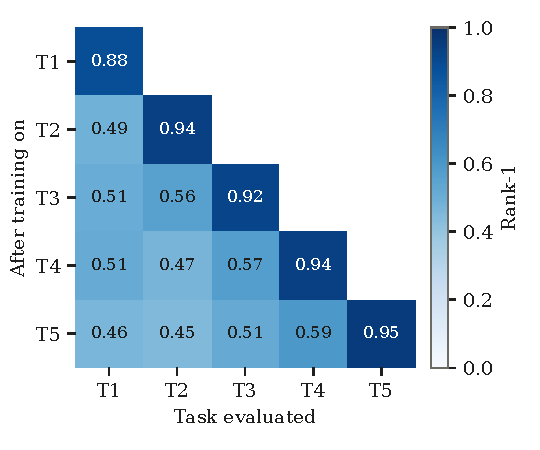
\includegraphics[width=0.58\textwidth]{acc_matrix_earvn_convnext.pdf}
\caption{Accuracy matrix $A[t][j]$ (rank-1) of naive training, EarVN1.0, ConvNeXt-T, seed 1. Row: after training on task $t$; column: task evaluated.}
\label{fig:matrix}
\end{figure}

Three cells just miss the rule because one seed is below 0.10: AWE ResNet-50 (mean 0.150), AWE MobileNetV3 (0.182) and AMI ResNet-50 (0.100). IITD forgets on the strict open-set threshold, not on rank-1: naive DIR@1\% forgetting is 0.18--0.22 for ResNet-50, DeiT-S and Swin-T. On AMI and IITD, with joint rank-1 at 0.97--1.00 and very similar photos of each person, there is little to forget on rank-1.

\subsection{Baselines}
Figure~\ref{fig:r2} compares naive training with the three reference methods. On EarVN, replay with only five images per person roughly halves forgetting in every family (a drop of 0.17--0.24), and LwF does as well or better without storing images: MobileNetV3 falls from 0.329 to 0.042 and ResNet-50 from 0.411 to 0.151. EWC helps less (0.27--0.36). So the forgetting in these cells can be reduced by known methods; it is not an artefact of the protocol.

\begin{figure}[H]
\centering
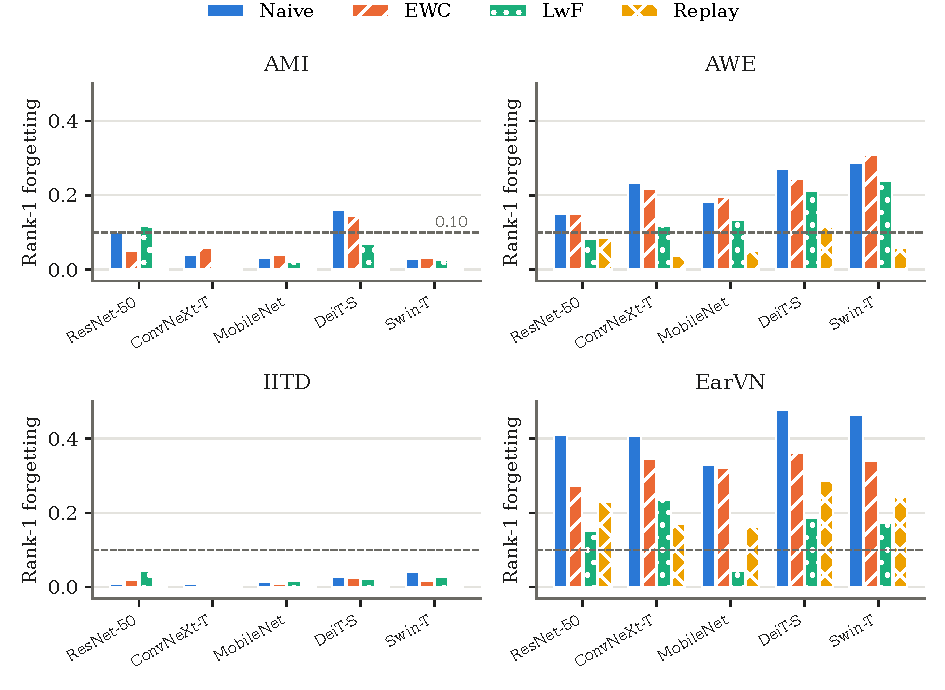
\includegraphics[width=\textwidth]{r2_forgetting.pdf}
\caption{R2: rank-1 forgetting of naive training and the three reference methods, mean over seeds. The dashed line is the 0.10 threshold of the R2 rule.}
\label{fig:r2}
\end{figure}

\noindent\textbf{Answer to RQ1.} Yes, on large data. Every model family forgets heavily when it learns EarVN's people in groups, and three of five do on AWE. On small, near-ceiling datasets forgetting on rank-1 is too small to pass the rule, though it can appear on strict open-set thresholds.

\section{The Nested Learning Arm}\label{sec:cms}
CMS is placed in the pointwise layers of every backbone, the layers that correspond to a Transformer's MLP (Table~\ref{tab:cmslayers}). Each such layer is replaced by three copies of its pretrained weights, combined by a learnable weighted sum, as in NL's independent variant initialised from a pretrained model (Figure~\ref{fig:cmslayer}):
\begin{equation}
y = \sum_{\ell=1}^{3} w_\ell \, \mathrm{MLP}^{(\ell)}(x), \qquad w = \mathrm{softmax}(a), \quad a \text{ initialised to } 0.
\end{equation}
At initialisation all copies are equal and the weights are $1/3$ each, so the CMS model computes exactly the pretrained model. The copies differ only through how often they update: copy~1 every step, copy~2 every 16 steps and copy~3 every 256 steps. A slow copy accumulates its gradients over its period and then takes one AdamW step, with learning rate $\eta \cdot C^{p}$ for its period $C$; the exponent $p \in \{0, 0.5\}$ was chosen per cell on seed 0. Everything else in the network updates every step.

\begin{table}[H]
\centering
\small
\caption{Layers replaced by CMS in each family.}
\label{tab:cmslayers}
\begin{tabular}{|l|l|c|}
\hline
\textbf{Family} & \textbf{Layers replicated} & \textbf{Count} \\
\hline
ResNet-50 & first and last 1$\times$1 conv of each bottleneck & 32 \\
ConvNeXt-T & MLP of each block & 18 \\
MobileNetV3 & pointwise expand / project convs & 29 \\
DeiT-S, Swin-T & MLP of each block & 12 \\
\hline
\end{tabular}
\end{table}

\begin{figure}[H]
\centering
\diagram{cms_layer}
\caption{The Nested Learning arm. Each pointwise layer of the backbone is replaced by three copies of its pretrained weights, updated at different frequencies and combined by learnable mixing weights.}
\label{fig:cmslayer}
\end{figure}

Unit tests check, for every family, that the CMS model equals the plain model at initialisation, that slow copies change only on their period, and that with all periods equal to 1 the copies stay identical.

\section{R3: Does CMS Reduce Forgetting? (RQ2)}
\subsection{Decision rule}
Naive + CMS is compared with naive on each cell, paired by seed. A cell is \emph{reduced} if (i) the mean forgetting drop is at least 0.05, (ii) CMS forgets less on every seed, or on all but one when there are five seeds, and (iii) mean final rank-1 is no more than 0.02 lower, so that CMS does not win by learning less. A reduced cell is also \emph{fixed} if its mean forgetting is below 0.10 and its final rank-1 is within 0.10 of joint. RQ2 is answered YES if more than half of the 9 shown cells are reduced, PARTIAL if at least one is, and NO otherwise.

\subsection{Results}
\textbf{RQ2: NO.} CMS reduced forgetting in none of the 9 cells (Table~\ref{tab:r3}).

\begin{table}[H]
\centering
\small
\caption{R3: naive + CMS against naive on the 9 cells with shown forgetting.}
\label{tab:r3}
\begin{tabular}{|l|c|c|c|c|c|}
\hline
\textbf{Cell} & \textbf{Naive} & \textbf{CMS} & \textbf{CMS better} & \textbf{Final rank-1} & \textbf{Verdict} \\
 & \textbf{forg.} & \textbf{forg.} & \textbf{(seeds)} & \textbf{change} & \\
\hline
AMI DeiT-S & 0.161 & 0.129 & 3 of 5 & $+0.037$ & not reduced \\
AWE ConvNeXt-T & 0.232 & 0.243 & 2 of 5 & $-0.026$ & not reduced \\
AWE DeiT-S & 0.271 & 0.250 & 2 of 5 & $+0.057$ & not reduced \\
AWE Swin-T & 0.286 & 0.296 & 2 of 5 & $-0.017$ & not reduced \\
EarVN ResNet-50 & 0.411 & 0.409 & 2 of 3 & $-0.007$ & not reduced \\
EarVN ConvNeXt-T & 0.407 & 0.371 & 3 of 3 & $+0.014$ & not reduced \\
EarVN MobileNetV3 & 0.329 & 0.312 & 3 of 3 & $+0.013$ & not reduced \\
EarVN DeiT-S & 0.476 & 0.479 & 1 of 3 & $-0.005$ & not reduced \\
EarVN Swin-T & 0.463 & 0.452 & 2 of 3 & $+0.010$ & not reduced \\
\hline
\end{tabular}
\end{table}

CMS neither helps nor hurts much: forgetting changes by less than 0.04 either way and final rank-1 by less than 0.06. The small effects lean positive on EarVN, where ConvNeXt-T and MobileNetV3 forget less on all three seeds, by 0.036 and 0.017, which is consistent but well short of 0.05. For comparison, LwF and replay lower EarVN forgetting by 0.17--0.29 on the same cells.

\subsection{Replay + CMS}
As a secondary comparison, CMS was added to replay and compared with replay alone, with the same test. It reduced forgetting in none of the 20 cells. The largest gain among the shown cells is AWE DeiT-S (0.114 to 0.064, better on 4 of 5 seeds), just under the threshold; AWE ConvNeXt-T gets worse (0.036 to 0.104). On EarVN, CMS lowers replay's forgetting by about 0.02 in four of five families.

\subsection{A known limit}
With fixed periods of 16 and 256 steps, the slowest copy updates only one to three times on AMI, AWE and IITD, and nine times on EarVN. The periods were fixed in advance for every cell, so on the small datasets the slow memory barely acts. This motivated the exploratory follow-up R4.

% ================================================================== CHAPTER 5
\chapter{Analysis: Why CMS Did Not Reduce Forgetting}\label{ch:analysis}

NL motivates CMS precisely as a remedy for forgetting, so its failure needs an explanation. This chapter reports diagnostics on one cell, then two exploratory variants that follow from them.

\section{Diagnostics}
Three runs of EarVN ConvNeXt-T, seed 1 (naive, R3 CMS and a task-aligned CMS from R4) were repeated with their weights saved after every task. In every run the reloaded weights reproduced the logged accuracies exactly. Four tests were made. They explain this one cell; they are not a measurement across the study.

\subsection{Where forgetting happens}
In the plain model (a rerun of the configuration in Figure~\ref{fig:matrix}, with weights saved), task~1 rank-1 falls from 0.885 to 0.493. Putting one part of the final model back to its weights after task~1 shows where the loss lies (Table~\ref{tab:restore}). Restoring the pointwise layers alone recovers 93\% of it. So CMS was placed exactly where the forgetting happens.

\begin{table}[H]
\centering
\small
\caption{Share of task-1 rank-1 loss recovered by restoring one part to its after-task-1 weights (EarVN ConvNeXt-T, seed 1).}
\label{tab:restore}
\begin{tabular}{|l|c|c|c|}
\hline
\textbf{Part restored} & \textbf{Naive} & \textbf{R3 CMS} & \textbf{R4 CMS} \\
\hline
Pointwise layers (all copies) & 93\% & -- & -- \\
Copy 1 (every step) & -- & 47\% & 69\% \\
Copy 2 & -- & 28\% & 5\% \\
Copy 3 & -- & 6\% & 5\% \\
Mixing weights & -- & 1\% & 1\% \\
Neck & 29\% & 25\% & 24\% \\
Rest of backbone & 18\% & 17\% & 24\% \\
\hline
\end{tabular}
\end{table}

With CMS, the forgetting moves into the fast copy: restoring copy~1 alone recovers 47\% (R3) and 69\% (R4), and the slow copies hold little.

\subsection{The slow copies barely learn}
Figure~\ref{fig:movement} shows how far each copy moved from its pretrained weights. After five tasks the fast copy has moved about 10\%, while the slowest copy has moved 1\% in R3 and 0.4\% in R4. Used alone, the slow copies score only 0.29--0.33 on the most recent task, against 0.85--0.89 for the fast copy. They learned little of the newest people, so they had little of the old ones to keep.

\begin{figure}[H]
\centering
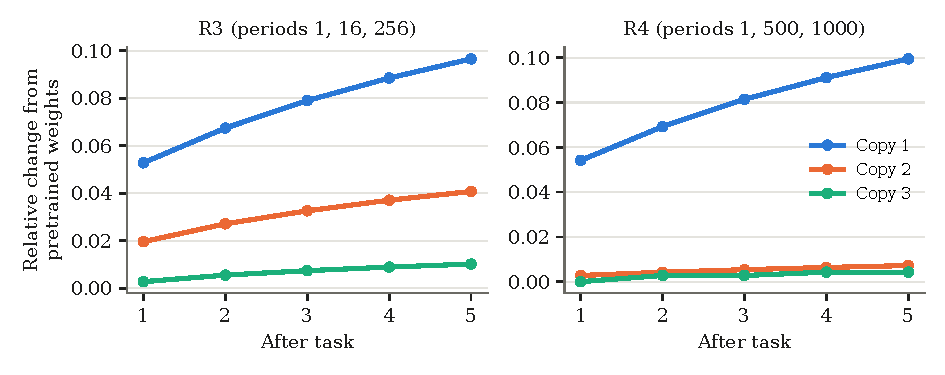
\includegraphics[width=\textwidth]{cms_copy_movement.pdf}
\caption{Relative L2 change of each CMS copy from its pretrained weights after each task (EarVN ConvNeXt-T, seed 1).}
\label{fig:movement}
\end{figure}

\subsection{Likely cause: the optimiser}
NL's update rule (Eq.~\ref{eq:cms}) applies the \emph{sum} of a period's gradients. With plain gradient descent this moves a period-$C$ copy about as far as $C$ ordinary steps. Here each slow level was stepped with AdamW, which normalises the update by running estimates of the gradient's magnitude, so one slow step moves about as far as one ordinary step and a period-$C$ copy learns roughly $1/C$ as much. The learning-rate exponent tried ($p \le 0.5$, a factor of at most $\sqrt{C}$) does not make up for this. Matching NL's rule would need $p = 1$ or plain gradient descent for the slow levels; neither was tested.

\subsection{Mixing weights}
The mean mixing weight of the fast copy grew from 0.333 to 0.388 (R3) and 0.398 (R4). The drift is small, and restoring the mixing weights changes task~1 by only 1\%, so the model is not routing around its slow memory; the slow memory is simply too weak.

\section{Exploratory Follow-ups}
Both follow-ups were designed after R3 had been seen, and were committed before their own runs. They use R3's test on the same 9 cells, with no correction for having looked at R3 first. Figure~\ref{fig:timelines} shows how the three CMS versions differ in when their slow copies change.

\begin{figure}[H]
\centering
\diagram{timelines}
\caption{When each copy changes over the five tasks, for EarVN ($S = 500$ steps per task). In R3 the slow copies take many small normalised steps; in R4 they step once per task or every two tasks; in R4b they take no gradient and are pulled towards the faster copy at task ends.}
\label{fig:timelines}
\end{figure}

\subsection{R4: task-aligned update periods}
The periods were tied to each cell's task length $S$: copy~1 every step, copy~2 every $S$ steps (once per task) and copy~3 every $2S$ steps, so the slow copies update five and two times on every dataset. R4 reduced forgetting in \textbf{2 of the 9 cells} and fixed none: AMI DeiT-S (0.161 to 0.100, better on 4 of 5 seeds) and EarVN ResNet-50 (0.411 to 0.353, all 3 seeds). Forgetting was lower than R3's in 8 of the 9 cells. Two reduced cells out of nine is a weak signal, since a few cells can pass a threshold by chance.

\subsection{R4b: consolidation at task boundaries}
Since the diagnostics showed that slow copies trained by gradient barely move, R4b gave them no gradient at all and instead moved knowledge down the chain at task boundaries, following NL's idea of explicit transfer between levels. Copy~1 trains every step. At the end of every task, copy~2 moves half-way towards copy~1; at the end of every second task, copy~3 first moves half-way towards copy~2:
\begin{equation}
\theta^{(3)} \leftarrow \theta^{(3)} + \beta\,(\theta^{(2)} - \theta^{(3)}), \qquad \theta^{(2)} \leftarrow \theta^{(2)} + \beta\,(\theta^{(1)} - \theta^{(2)}), \qquad \beta = 0.5.
\end{equation}
R4b reduced forgetting in \textbf{none of the 9 cells}. Its largest drop is 0.029 (AMI DeiT-S), and on EarVN DeiT-S and Swin-T it forgets more than naive. At the end, the fast copy's mixing weight is 0.37--0.45 on the EarVN CNNs: the copies that hold old knowledge are partly switched off, and since they take no gradient they cannot push back. With $\beta = 0.5$, copy~2 also keeps only $0.5^4 \approx 6\%$ of what it held after task~1 by the end of five tasks.

\begin{figure}[H]
\centering
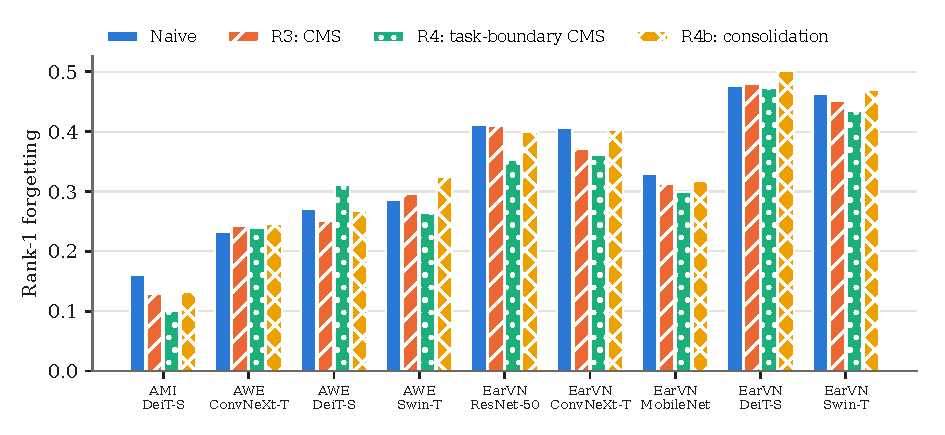
\includegraphics[width=\textwidth]{cms_forgetting.pdf}
\caption{Rank-1 forgetting on the 9 cells with shown forgetting: naive training and the three CMS variants (mean over seeds).}
\label{fig:cms}
\end{figure}

\begin{table}[H]
\centering
\small
\caption{Summary of the CMS variants on the 9 cells with shown forgetting.}
\label{tab:variants}
\begin{tabular}{|l|l|c|c|}
\hline
\textbf{Stage} & \textbf{Variant} & \textbf{Reduced} & \textbf{Fixed} \\
\hline
R3 (pre-registered) & CMS, periods 1, 16, 256 & 0 of 9 & 0 \\
R3 secondary & Replay + CMS vs.\ replay & 0 of 20 & 0 \\
R4 (exploratory) & CMS, periods 1, $S$, $2S$ & 2 of 9 & 0 \\
R4b (exploratory) & Consolidation, $\beta = 0.5$ & 0 of 9 & 0 \\
\hline
\end{tabular}
\end{table}

% ================================================================== CHAPTER 6
\chapter{Conclusions}\label{ch:conclusions}

\section{Answers to the Research Questions}
\begin{itemize}
\item \textbf{RQ1: yes, on large data.} All five model families forget heavily when they learn EarVN's people in groups (rank-1 forgetting 0.33--0.48), and three of five do on AWE. Near-ceiling datasets (AMI, IITD) hide forgetting on rank-1. Forgetting does not depend on whether the model is a CNN or a transformer.
\item \textbf{RQ2: no.} Under a rule fixed before the runs, CMS in the pointwise layers reduced forgetting in none of the 9 cells, and adding it to replay helped in none of 20. Simple baselines (LwF, replay) do far better on the same cells.
\item \textbf{RQ3: not yet.} Of two exploratory variants, task-aligned periods came closest (2 of 9 cells reduced), and explicit consolidation did not help. The diagnostics show what a working version would need: slow levels that actually accumulate what the fast level learns.
\end{itemize}

\section{Novelty and Contributions}
The study gives a pre-registered, multi-family benchmark of continual ear recognition, the first test of Nested Learning's CMS on vision backbones and biometrics, and diagnostics that separate where forgetting happens from why the memory designed to stop it did not. A negative result with a located cause is useful: it tells the next experiment what to change.

\section{Assumptions and Limitations}
\begin{itemize}
\item \textbf{UERC is not included.} The largest dataset, which would test the result at scale, did not finish in time.
\item \textbf{Few seeds on EarVN} (three) and \textbf{tiny per-task tests on AMI and AWE}, where one probe moves a task's rank-1 by 0.07.
\item \textbf{EarVN recipes sit at the corner of the R1 grid,} so longer training could change how much is forgotten.
\item \textbf{One CMS placement and one aggregation.} Only the independent variant in the pointwise layers was tested, not chained or nested CMS, and not CMS in the neck.
\item \textbf{The diagnostics cover one model, one dataset and one seed.}
\item \textbf{R4 and R4b are exploratory:} they were designed after R3 was seen and need confirmation on fresh seeds.
\item \textbf{Compute:} all runs were on Kaggle T4 GPUs within session limits, which bounded the grids.
\end{itemize}

\section{Future Scope}
\begin{itemize}
\item \textbf{Fix the slow-level update.} Step slow levels with the full summed gradient, either with plain gradient descent or with a learning rate scaled by the period ($p = 1$), as NL's rule implies.
\item \textbf{Better consolidation.} A smaller $\beta$, or fixed mixing weights, so that consolidated copies are neither overwritten nor switched off.
\item \textbf{Other placements,} such as CMS in the embedding neck, and the chained and nested variants.
\item \textbf{UERC 2023,} to test all results at the scale of a thousand identities.
\item \textbf{Combining CMS with LwF,} the strongest replay-free method here, for continual enrollment without storing biometric images.
\end{itemize}

% ================================================================== BIBLIOGRAPHY
\begin{thebibliography}{99}

\bibitem{behrouz2025nested}
A.~Behrouz, M.~Razaviyayn, P.~Zhong, and V.~Mirrokni, ``Nested learning: The illusion of deep learning architectures,'' in \emph{Advances in Neural Information Processing Systems (NeurIPS)}, 2025.

\bibitem{behrouz2025titans}
A.~Behrouz, P.~Zhong, and V.~Mirrokni, ``Titans: Learning to memorize at test time,'' \emph{arXiv preprint arXiv:2501.00663}, 2025.

\bibitem{mccloskey1989}
M.~McCloskey and N.~J. Cohen, ``Catastrophic interference in connectionist networks: The sequential learning problem,'' \emph{Psychology of Learning and Motivation}, vol.~24, pp.~109--165, 1989.

\bibitem{delange2021survey}
M.~De~Lange, R.~Aljundi, M.~Masana, S.~Parisot, X.~Jia, A.~Leonardis, G.~Slabaugh, and T.~Tuytelaars, ``A continual learning survey: Defying forgetting in classification tasks,'' \emph{IEEE Transactions on Pattern Analysis and Machine Intelligence}, vol.~44, no.~7, pp.~3366--3385, 2022.

\bibitem{vandeven2019three}
G.~M. van~de~Ven and A.~S. Tolias, ``Three scenarios for continual learning,'' \emph{arXiv preprint arXiv:1904.07734}, 2019.

\bibitem{kirkpatrick2017ewc}
J.~Kirkpatrick \emph{et al.}, ``Overcoming catastrophic forgetting in neural networks,'' \emph{Proceedings of the National Academy of Sciences}, vol.~114, no.~13, pp.~3521--3526, 2017.

\bibitem{li2017lwf}
Z.~Li and D.~Hoiem, ``Learning without forgetting,'' \emph{IEEE Transactions on Pattern Analysis and Machine Intelligence}, vol.~40, no.~12, pp.~2935--2947, 2018.

\bibitem{rebuffi2017icarl}
S.-A. Rebuffi, A.~Kolesnikov, G.~Sperl, and C.~H. Lampert, ``iCaRL: Incremental classifier and representation learning,'' in \emph{Conference on Computer Vision and Pattern Recognition (CVPR)}, 2017.

\bibitem{chaudhry2019tiny}
A.~Chaudhry, M.~Rohrbach, M.~Elhoseiny, T.~Ajanthan, P.~K. Dokania, P.~H.~S. Torr, and M.~Ranzato, ``On tiny episodic memories in continual learning,'' \emph{arXiv preprint arXiv:1902.10486}, 2019.

\bibitem{chaudhry2018riemannian}
A.~Chaudhry, P.~K. Dokania, T.~Ajanthan, and P.~H.~S. Torr, ``Riemannian walk for incremental learning: Understanding forgetting and intransigence,'' in \emph{European Conference on Computer Vision (ECCV)}, 2018.

\bibitem{lopezpaz2017gem}
D.~Lopez-Paz and M.~Ranzato, ``Gradient episodic memory for continual learning,'' in \emph{Advances in Neural Information Processing Systems (NeurIPS)}, 2017.

\bibitem{emersic2017survey}
{\v Z}.~Emer{\v s}i{\v c}, V.~{\v S}truc, and P.~Peer, ``Ear recognition: More than a survey,'' \emph{Neurocomputing}, vol.~255, pp.~26--39, 2017.

\bibitem{emersic2023uerc}
{\v Z}.~Emer{\v s}i{\v c} \emph{et al.}, ``The unconstrained ear recognition challenge 2023: Maximizing performance and minimizing bias,'' in \emph{IEEE International Joint Conference on Biometrics (IJCB)}, 2023.

\bibitem{gonzalez2012ami}
E.~Gonzalez, L.~Alvarez, and L.~Mazorra, ``Normalization and feature extraction on ear images,'' in \emph{IEEE International Carnahan Conference on Security Technology (ICCST)}, 2012.

\bibitem{kumar2012iitd}
A.~Kumar and C.~Wu, ``Automated human identification using ear imaging,'' \emph{Pattern Recognition}, vol.~45, no.~3, pp.~956--968, 2012.

\bibitem{hoang2019earvn}
V.~T. Hoang, ``EarVN1.0: A new large-scale ear images dataset in the wild,'' \emph{Data in Brief}, vol.~27, 104630, 2019.

\bibitem{deng2019arcface}
J.~Deng, J.~Guo, N.~Xue, and S.~Zafeiriou, ``ArcFace: Additive angular margin loss for deep face recognition,'' in \emph{Conference on Computer Vision and Pattern Recognition (CVPR)}, 2019.

\bibitem{he2016resnet}
K.~He, X.~Zhang, S.~Ren, and J.~Sun, ``Deep residual learning for image recognition,'' in \emph{Conference on Computer Vision and Pattern Recognition (CVPR)}, 2016.

\bibitem{liu2022convnext}
Z.~Liu, H.~Mao, C.-Y. Wu, C.~Feichtenhofer, T.~Darrell, and S.~Xie, ``A ConvNet for the 2020s,'' in \emph{Conference on Computer Vision and Pattern Recognition (CVPR)}, 2022.

\bibitem{howard2019mobilenetv3}
A.~Howard \emph{et al.}, ``Searching for MobileNetV3,'' in \emph{International Conference on Computer Vision (ICCV)}, 2019.

\bibitem{touvron2021deit}
H.~Touvron, M.~Cord, M.~Douze, F.~Massa, A.~Sablayrolles, and H.~J{\'e}gou, ``Training data-efficient image transformers \& distillation through attention,'' in \emph{International Conference on Machine Learning (ICML)}, 2021.

\bibitem{liu2021swin}
Z.~Liu, Y.~Lin, Y.~Cao, H.~Hu, Y.~Wei, Z.~Zhang, S.~Lin, and B.~Guo, ``Swin Transformer: Hierarchical vision transformer using shifted windows,'' in \emph{International Conference on Computer Vision (ICCV)}, 2021.

\bibitem{loshchilov2019adamw}
I.~Loshchilov and F.~Hutter, ``Decoupled weight decay regularization,'' in \emph{International Conference on Learning Representations (ICLR)}, 2019.

\bibitem{wightman2019timm}
R.~Wightman, ``PyTorch image models,'' GitHub repository, \url{https://github.com/huggingface/pytorch-image-models}, 2019.

\end{thebibliography}

\end{document}
